%************************************************
\chapter{Introduction}\label{ch:introduction}
%************************************************
Functional programming languages are an alternative to the classical imperative paradigm. While imperative programs act on the state of the machine, functional ones are stateless, without any side effect. Functions, indeed, are intended as in mathematics. Unlike procedures, a function called with the same argument always returns the same result, i.e. referential transparency holds. This way, formal reasoning about programs, for example operated by compilers, is easier, since the context does not need to be considered \cite{backus_can_1978}. Moreover functional programs are typically more concise than their imperative counterpart. Typical features of functional programming languages, such as higher-order functions, algebraic data types and pattern matching, in fact ease the process of writing generic and abstract code, thus allowing modularity and code reuse. Then, why are they used so little? One of the reasons is certainly performances. The model of computation underlying functional programs is in fact very different from the hardware devoted to their execution and this gap can lead to a massive performance loss. This way, compilers become crucial in the process of software development, since depending on the type of translation they operate, the resulting machine code can be very different. In particular, in pure functional programs, different orders of evalution of functions lead to the same result, because of the absence of side effects. However this order is fixed by compilers which operate a choice fundamental with respect to performances. Studying these phenomena directly on real programming languages and compilers is very hard. Indeed, one needs to consider some abstract models of computation. Since functional programming languages are the target, it seems natural to study their mechanisms in the context of the $\lambda$-calculus. The $\lambda$-calculus in fact is a very good model for functional languages, and in particular it allows a fine analysis of function calling mechanisms \cite{plotkin_call-by-name_1975}. Moreover, $\lambda$-calculus itself can be seen as an instance of an \emph{abstract reduction system}, a wider class of models used to study \emph{rewriting systems} in the abstract. This way, a lot of results in the abstract theory of rewriting can be directly applied to the $\lambda$-calculus. In this thesis we introduce for the first time the notion of randomised strategy in the scope of the $\lambda$-calculus. We give an informal motivating example which justifies our interest.
\begin{example}
	Let us consider the situation depicted in Figure~\ref{figure:intro}. In the initial state we are in $S$ and we want to reach $A$ in the minimum number of steps. We can go either left or right. In both cases another decision has to be taken at the second step, again if we want to go left or right.
\end{example}
\begin{figure}
	\centering
	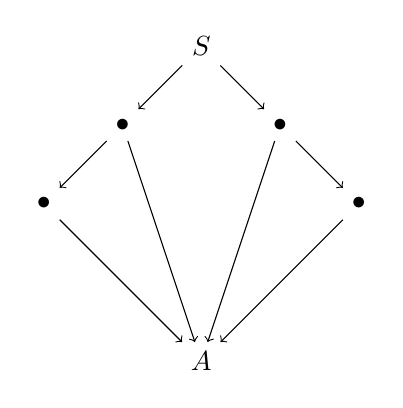
\begin{tikzpicture}
		[node distance=20mm, auto, transform shape]
		\node (S) at (0,0) {$S$};
		\node (n) at (-1,-1) {$\bullet$};
		\node (l) at (1,-1) {$\bullet$};
		\node (r) at (-2,-2) {$\bullet$};
		\node (s) at (2,-2) {$\bullet$};
		\node (A) at (0,-4) {$A$};
		\draw (S) edge[->] node[left=5pt] {} (n);
		\draw (S) edge[->] node[right=5pt] {} (l);
		\draw (n) edge[->] node[left=5pt] {} (A);
		\draw (l) edge[->] node[right=5pt] {} (A);
		\draw (n) edge[->] node[right=5pt] {} (r);
		\draw (l) edge[->] node[right=5pt] {} (s);
		\draw (r) edge[->] node[right=5pt] {} (A);
		\draw (s) edge[->] node[right=5pt] {} (A);
	\end{tikzpicture}
	\caption{Introductory example}
	\label{figure:intro}
\end{figure}
%*****************************************
